\documentclass{article}
\usepackage{epsfig, latexsym}

\begin{document}

\newcommand{\bs}{\backslash}

\title{
\Huge{CMPEN 271 -- Spring 2012}\\
\normalsize{Exam 2}\\
\makebox[4in][l]{Name:}
PSU ID:}
\date{}

\maketitle{}

\begin{tabular}{llll}
\begin{tabular}{c||c}
D & Q+   \\ \hline
0 & 0 \\ \hline
1 & 1 \\
\end{tabular}
&
\begin{tabular}{c||c}
T & Q+   \\ \hline
0 & Q \\ \hline
1 & Q' \\
\end{tabular}
&
\begin{tabular}{c|c||c}
S & R & Q+   \\ \hline
0 & 0 & Q \\ \hline
0 & 1 & 0 \\ \hline
1 & 0 & 1 \\ \hline
1 & 1 & x \\
\end{tabular}
&
\begin{tabular}{c|c||c}
J & K & Q+   \\ \hline
0 & 0 & Q \\ \hline
0 & 1 & 0 \\ \hline
1 & 0 & 1 \\ \hline
1 & 1 & Q' \\
\end{tabular}
\end{tabular}


\begin{enumerate}
\item {($1*10^{-6}$ pt.)} Assuming a word size of 5 bits, interpret 10100 as a 2's complement
number.

\begin{tabular}{p{0.6in} p{0.6in} p{0.6in} p{0.6in} l}
a) -24 & b) -12 & c) -6 & d) -2 & e) None of the above.
\end{tabular}

\item {($1*10^{-6}$ pt.)} Assuming a word size of 4 bits, determine the 2's complement
representation of -7.

\begin{tabular}{p{0.6in} p{0.6in} p{0.6in} p{0.6in} l}
a) 1011 & b) 1101 & c) 1100 & d) 1001 & e) None of the above.
\end{tabular}

\item {($1*10^{-6}$ pt.)} An If/Then statement represents which piece of hardware?

\begin{tabular}{p{0.8in} p{0.6in} p{0.9in} p{0.8in} l}
a) decoder & b) mux & c) comparator & d) counter & e) register
\end{tabular}

\item {($1*10^{-6}$ pt.)} How many 2:1 muxes are needed to construct a 4-bit wide
4:1 mux?

\begin{tabular}{p{0.6in} p{0.6in} p{0.6in} p{0.6in} l}
a) 8 & b) 12 & c) 18 & d) 24 & e) None of the above.
\end{tabular}

\pagebreak
Questions 5-7 concern the construction of a bit-slice of a comparator.  The questions 
will ask you to complete the entries in the truth table below denoted by $a$, $b$, and
$c$.

\begin{tabular}{l|l|l|l|l||l|l|l}
$G_{in}$ & $L_{in}$ & $E_{in}$ & $x$ & $y$ & $G_{out}$ & $L_{out}$ & $E_{out}$ \\ \hline
    0    &    0     &     1    &  1  &  0  &   $a$     &           &           \\ \hline
    0    &    1     &     0    &  1  &  0  &           &   $b$     &           \\ \hline
    1    &    0     &     1    &  1  &  0  &           &           &    $c$    \\
\end{tabular}

\item {($1*10^{-6}$ pt.)}What is the value of $a$?

\begin{tabular}{p{0.6in} p{0.6in} p{0.6in}}
a) 0 & b) 1 & c) x 
\end{tabular}

\item {($1*10^{-6}$ pt.)}What is the value of $b$?

\begin{tabular}{p{0.6in} p{0.6in} p{0.6in}}
a) 0 & b) 1 & c) x 
\end{tabular}

\item {($1*10^{-6}$ pt.)}What is the value of $c$?

\begin{tabular}{p{0.6in} p{0.6in} p{0.6in}}
a) 0 & b) 1 & c) x 
\end{tabular} \\

For questions 8-11 use the following figure

\scalebox{0.7}{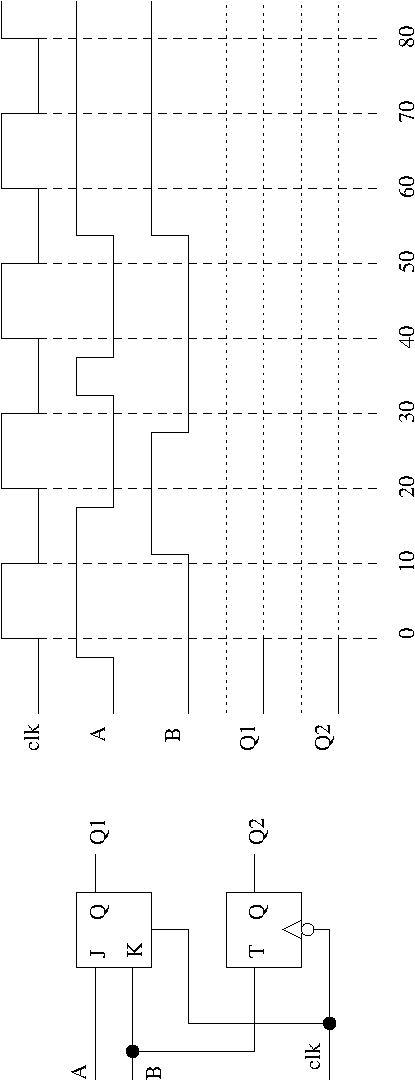
\includegraphics[angle=-90]{./Fig2/ExTim3}}

\item {($1*10^{-6}$ pt.)} What is the value of Q1 at time 45

\begin{tabular}{p{0.75in}p{0.75in}p{1.75in}}
a) 0 & b) 1 & c) toggling \\
\end{tabular}

\item {($1*10^{-6}$ pt.)} What is the value of Q1 at time 65

\begin{tabular}{p{0.75in}p{0.75in}p{1.75in}}
a) 0 & b) 1 & c) toggling \\
\end{tabular}

\item {($1*10^{-6}$ pt.)} What is the value of Q2 at time 25

\begin{tabular}{p{0.75in}p{0.75in}p{1.75in}}
a) 0 & b) 1 & c) toggling \\
\end{tabular}

\item {($1*10^{-6}$ pt.)} What is the value of Q2 at time 75

\begin{tabular}{p{0.75in}p{0.75in}p{1.75in}}
a) 0 & b) 1 & c) toggling \\
\end{tabular}

\pagebreak
You have a digital design which calls for a circuit to perform the 
following task.

\begin{verbatim}
if      (sum > 18) z = sum-18
else if (sum > 12) z = sum-12
else if (sum > 6)  z = sum-6
else               z = sum
\end{verbatim}

You have decided on the architecture shown below.  
Its your job to design to complete the truth table
for the the glue-logic box (only an arbitrary portion of the complete 
truth table is shown).  


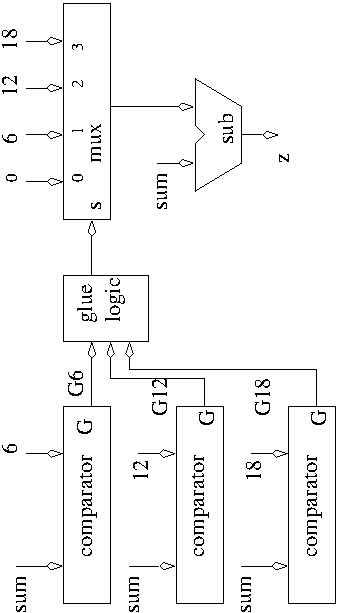
\includegraphics[angle=-90]{./Fig2/if8}

\vspace{0.25in}

\begin{tabular}{l|l|l||l}
G6 & G12 & G18 & select \\ \hline
1  & 1   & 0   &   a   \\ \hline
1  & 0   & 0   &   b   \\ \hline
1  & 1   & 1   &   c   \\ 
\end{tabular}

\vspace{0.25in}

\item {($1*10^{-6}$ pt.)}What is the (decimal) value of a in the truth table?

\begin{tabular}{p{0.6in} p{0.6in} p{0.6in} p{0.6in} l}
a) 0 & b) 1 & c) 2 & d) 3 & e) x  
\end{tabular}

\item {($1*10^{-6}$ pt.)}What is the (decimal) value of b in the truth table?

\begin{tabular}{p{0.6in} p{0.6in} p{0.6in} p{0.6in} l}
a) 0 & b) 1 & c) 2 & d) 3 & e) x  
\end{tabular}

\item {($1*10^{-6}$ pt.)}What is the (decimal) value of c in the truth table?

\begin{tabular}{p{0.6in} p{0.6in} p{0.6in} p{0.6in} l}
a) 0 & b) 1 & c) 2 & d) 3 & e) x  
\end{tabular}

\pagebreak
For questions 15,17 assume that a 4-bit up/down counter with parallel load
has the following truth table.   Complete the timing diagram below.

\begin{tabular}{l|l|l||l|l}
clk             & $c$		& D & $Q^+$ & roll  \\ \hline
0,1,$\downarrow$& xx            & x & Q     & 1 if Q=15 and c=01 \\ \hline
$\uparrow$      & 00            & x & Q     & 0			 \\  \hline
$\uparrow$      & 01            & x & $Q+1$ & 1 if Q=15 and c=01 \\ \hline
$\uparrow$      & 10            & x & $Q-1$ & 0			\\  \hline
$\uparrow$      & 11            & D & D     & 0			 \\
\end{tabular}

\scalebox{0.7}{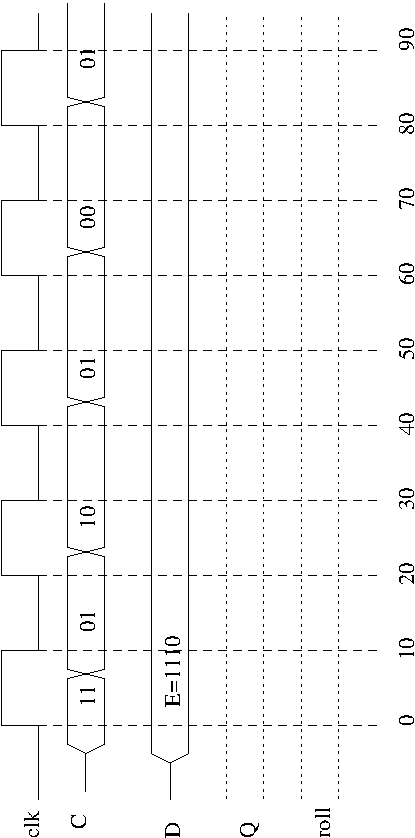
\includegraphics[angle=-90]{./Fig2/count-time2}}

\item {($1*10^{-6}$ pt.)}What is the value of $Q$ at time 55?

\begin{tabular}{p{0.6in} p{0.6in} p{0.6in} p{0.6in} l}
a) 0000 & b) 0001 & c) 1110 & d) 1111 & e) none of the above
\end{tabular}

\item {($1*10^{-6}$ pt.)}What is the value of $Q$ at time 90?

\begin{tabular}{p{0.6in} p{0.6in} p{0.6in} p{0.6in} l}
a) 0000 & b) 0001 & c) 1110 & d) 1111 & e) none of the above
\end{tabular}


\item {($1*10^{-6}$ pt.)}At which of the following times does roll=1

\begin{tabular}{p{0.6in} p{0.6in} p{0.6in} p{0.6in} l}
a) 30 & b) 50 & c) 70 & d) 90 & e) none of the above
\end{tabular}



\pagebreak
You have a digital design which calls for a circuit
to perform the following task.  

\begin{verbatim}
for (i=0; i<42; i++) total = 2*total + i
\end{verbatim}

You have decided on the architecture shown below.  Its your job to 
finish the design. The box labeled "times 2" multiplies its input
by 2 and outputs this value.

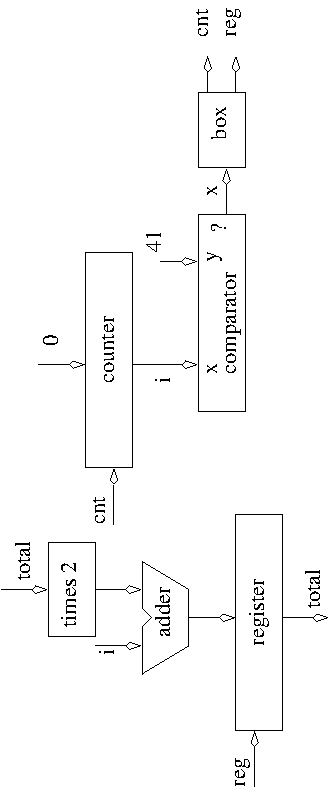
\includegraphics[angle=-90]{./Fig2/combo6}

\item {($1*10^{-6}$ pt.)}Which output of the comparator should be connected
to the input of "box"?

\begin{tabular}{p{0.6in} p{0.6in} p{0.6in} l}
a) G & b) L & c) E & d) none of the above.  
\end{tabular}

\item {($1*10^{-6}$ pt.)}Assume that the counter has the truth table
which is the same as question 15-17.  What is the logic inside "box"
to control the counter?  Note, the output of the comparator is called "x."

\begin{description}
\item{a) } $cnt_1 = 0$ and $cnt_0 = 0$
\item{b) } $cnt_1 = x'$ and $cnt_0 = 0$
\item{c) } $cnt_1 = 0$ and $cnt_0 = x'$
\item{d) } $cnt_1 = x$ and $cnt_0 = x'$
\item{e) } None of the above.
\end{description}

\item {($1*10^{-6}$ pt.)}How many logic gates are required in the "times 2" box?

\begin{tabular}{p{0.6in} p{0.6in} p{0.6in} p{0.6in} l}
a) none & b) a few & c) some & d) a lot & e) infinite  
\end{tabular}

\pagebreak
For problems 21-25 use the following figure and timing diagram.

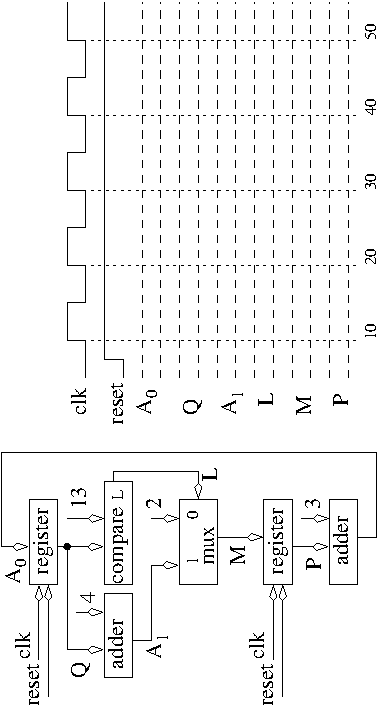
\includegraphics[angle=-90]{./Fig2/BBBtiming3}

\item {($2*10^{-6}$ pts.)}What is the value of $P$ at time 15?

\begin{tabular}{p{0.6in} p{0.6in} p{0.6in} p{0.6in} l}
a) 0  & b) 3  & c) 4  & d) 6  & e)  11
\end{tabular}

\item {($2*10^{-6}$ pts.)}What is the value of $A_0$ at time 25?

\begin{tabular}{p{0.6in} p{0.6in} p{0.6in} p{0.6in} l}
a) 3  & b) 5  & c) 7  & d) 8 & e) 10
\end{tabular}

\item {($2*10^{-6}$ pts.)}What is the value of $A_1$ at time 35?

\begin{tabular}{p{0.6in} p{0.6in} p{0.6in} p{0.6in} l}
a) 8  & b) 11  & c) 14 & d) 15  & e) 18
\end{tabular}

\item {($2*10^{-6}$ pts.)}What is the value of $Q$ at time 45?

\begin{tabular}{p{0.6in} p{0.6in} p{0.6in} p{0.6in} l}
a) 5  & b) 7  & c) 11 & d) 13  & e) 14
\end{tabular}

\item {($2*10^{-6}$ pts.)}What is the value of $M$ at time 55?

\begin{tabular}{p{0.6in} p{0.6in} p{0.6in} p{0.6in} l}
a) 2  & b) 5  & c) 7 & d) 8  & e) 9
\end{tabular}
\end{enumerate}
\end{document}
